\section{Zadanie 14}
Rozważ spacer losowy po grafie przedstawionym na rysunku.
Spacer startuje z wierzchołka A.
Rozważ stowarzyszony z nim łańcuch Markowa $(X_n)_{n\in \mathbb{N}}$,
gdzie stanami są wuerzchołki grafu oraz $X_0 = A$.
\begin{enumerate}[label=(\roman*)]
    \item\label{set07.task14.1} Wyznacz $\lim_{n\to\infty} P(X_n = A)$ oraz $\lim_{n\to\infty} P(X_n = B)$.
    \item\label{set07.task14.2} Jaka jest oczekiwana liczba odwiedzin wierzchołka B przed pierwszym powrotem do A?
\end{enumerate}
\begin{center}
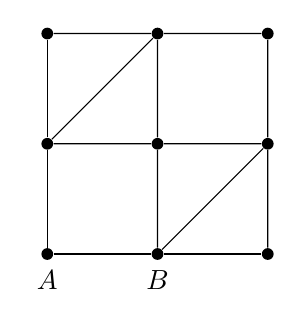
\begin{tikzpicture}[scale=1.4]

    % Wierzchołki
    \node (A) at (0,0) [circle,fill,inner sep=1.5pt,label=below:$A$] {};
    \node (B) at (1,0) [circle,fill,inner sep=1.5pt,label=below:$B$] {};
    \node (C) at (2,0) [circle,fill,inner sep=1.5pt] {};
    
    \node (D) at (0,1) [circle,fill,inner sep=1.5pt] {};
    \node (E) at (1,1) [circle,fill,inner sep=1.5pt] {};
    \node (F) at (2,1) [circle,fill,inner sep=1.5pt] {};
    
    \node (G) at (0,2) [circle,fill,inner sep=1.5pt] {};
    \node (H) at (1,2) [circle,fill,inner sep=1.5pt] {};
    \node (I) at (2,2) [circle,fill,inner sep=1.5pt] {};
    
    % Krawędzie poziome
    \draw (A) -- (B) -- (C);
    \draw (D) -- (E) -- (F);
    \draw (G) -- (H) -- (I);
    
    % Krawędzie pionowe
    \draw (A) -- (D) -- (G);
    \draw (B) -- (E) -- (H);
    \draw (C) -- (F) -- (I);
    
    % Przekątne
    \draw (D) -- (H); % górny lewy kwadrat
    \draw (B) -- (F); % dolny prawy kwadrat
    
\end{tikzpicture}
\end{center}

\subsection*{Rozwiązanie podpunktu \ref{set07.task14.1}}
Łańcuch jest skończony, spójny i aperiodyczny 
(w grafie są trójkąty i kwadraty, więc okres $= gcd(3, 4) = 1$) więc dla każdego puktu $Q$ 
$P(X_n = Q)$ zbiega do rozkładu stacjonarnego $\pi$.
Dla losowego spaceru po grafie rozkład stacjonarny ma postać:

\[
\pi(v)=\frac{\deg(v)}{\sum_{u}\deg(u)}.
\]

Wierzchołki narożne mają stopień $2$, pozostałe pięć
wierzchołków ma stopień $4$. Suma stopni:

\[
4\cdot 2 + 5\cdot 4 = 28.
\]

Więc

\[
\pi(A)=\frac{\deg(A)}{28}=\frac{2}{28}=\frac{1}{14}, 
\qquad
\pi(B)=\frac{\deg(B)}{28}=\frac{4}{28}=\frac{1}{7}.
\]

Czyli:

\[
\lim_{n\to\infty} P(X_n = A) = \frac{1}{14},
\qquad
\lim_{n\to\infty} P(X_n = B) = \frac{1}{7}.
\]

\subsection*{Rozwiązanie podpunktu \ref{set07.task14.2}}
Oczekiwana liczba odwiedzeń wierzchołka $B$ przed powrotem do $A$ to po prostu
stosunek średniej liczby odwiedzin $B$ do odwiedzin $A$ w długim czasie ($n\to\infty$), 
który jest równy:

\[
\frac{\pi(B)}{\pi(A)}
= \frac{1/7}{1/14}
= 2.
\]

\subsection*{Odpowiedź}
\[
\boxed{
    \text{(i)} 
        \lim_{n\to\infty} P(X_n = A) = \frac{1}{14},
        \qquad
        \lim_{n\to\infty} P(X_n = B) = \frac{1}{7}
        \qquad
    \text{(ii)} 
        \qquad 
        2
    }
\]
